%\documentclass[11pt,a4paper]{article}
\documentclass[preview]{standalone}
\usepackage[utf8]{inputenc}
\usepackage{graphicx}
\usepackage{subcaption}
\newcommand{\figures}{./figure}

\begin{document}

\begin{figure}
    \centering
    \begin{subfigure}[b]{0.45\textwidth}
        \caption{}
        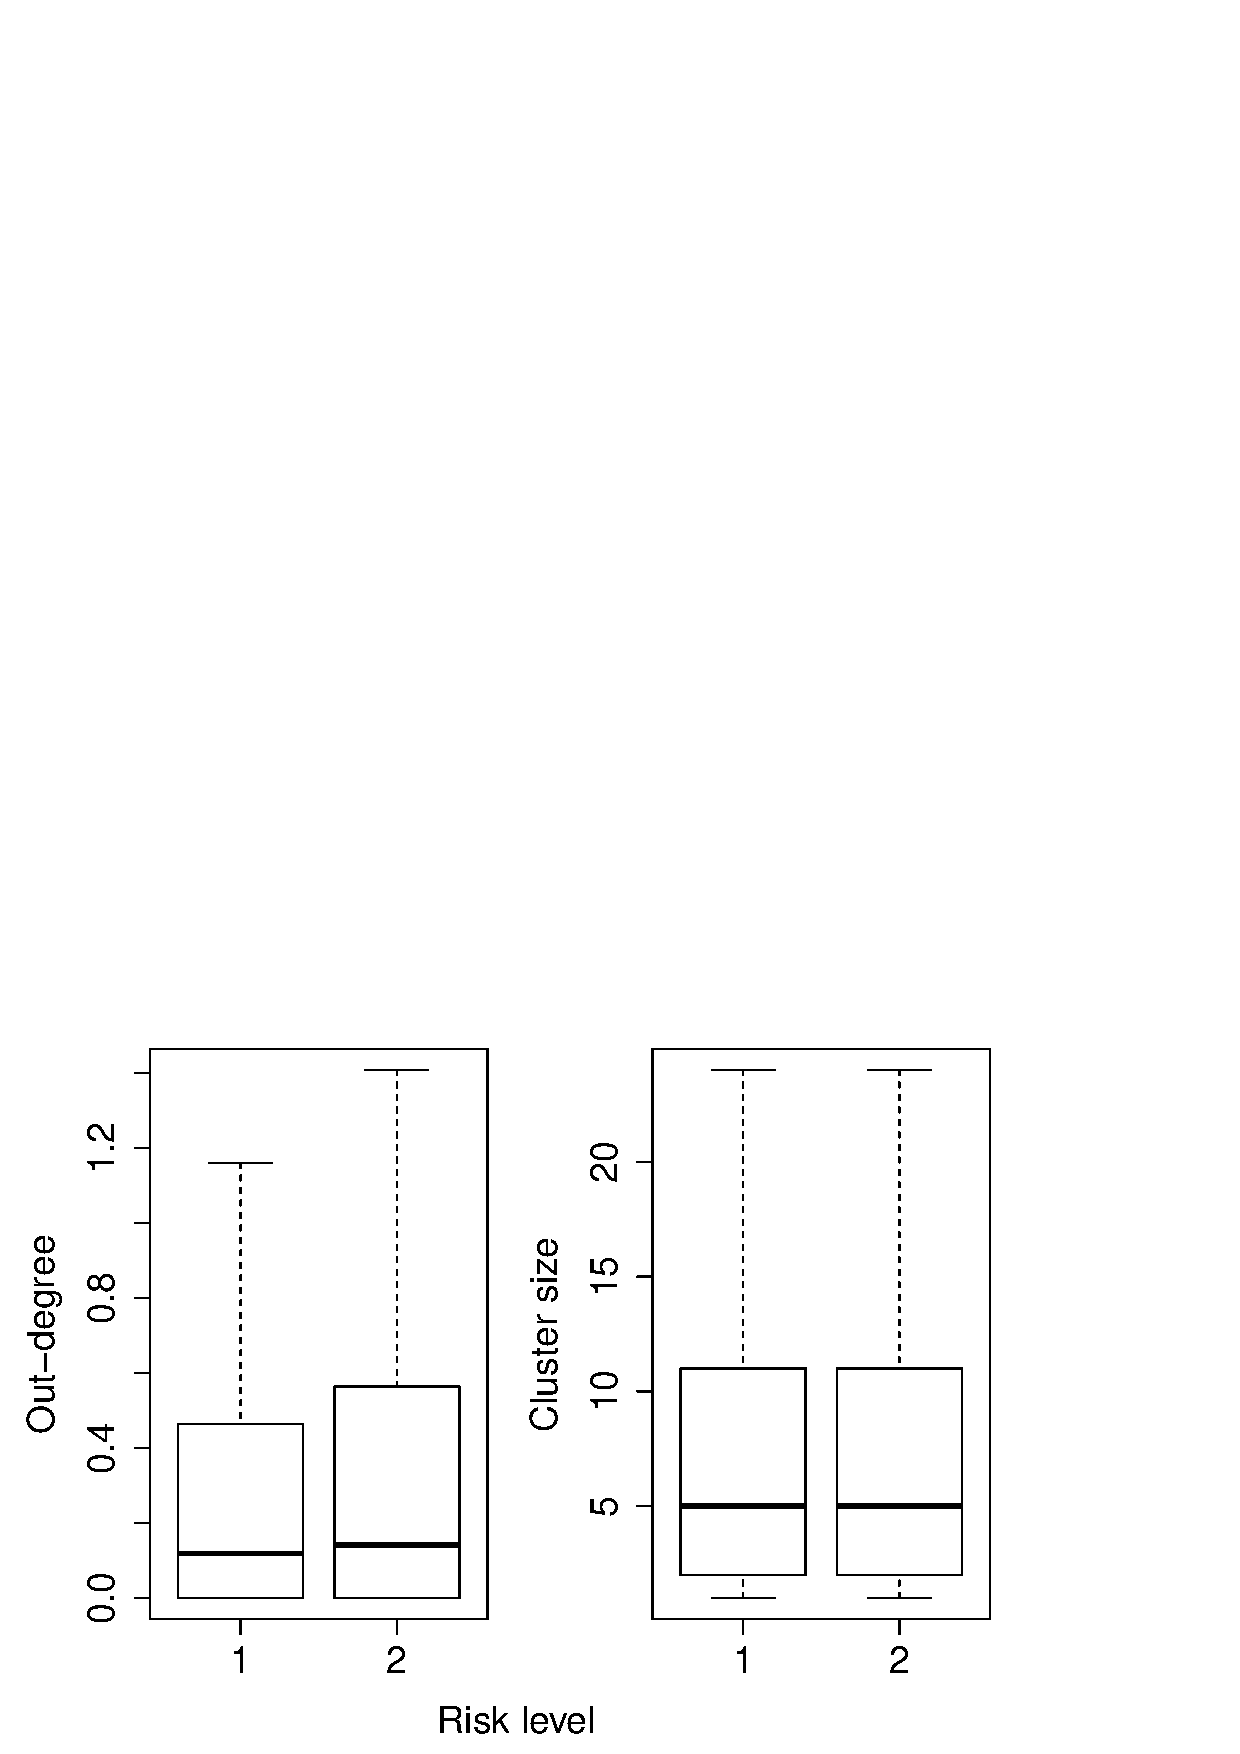
\includegraphics[width=\textwidth]{\figures/bp_base-1.pdf}
        \label{fig1a}
    \end{subfigure}
    ~ 
    \begin{subfigure}[b]{0.45\textwidth}
        \caption{}
        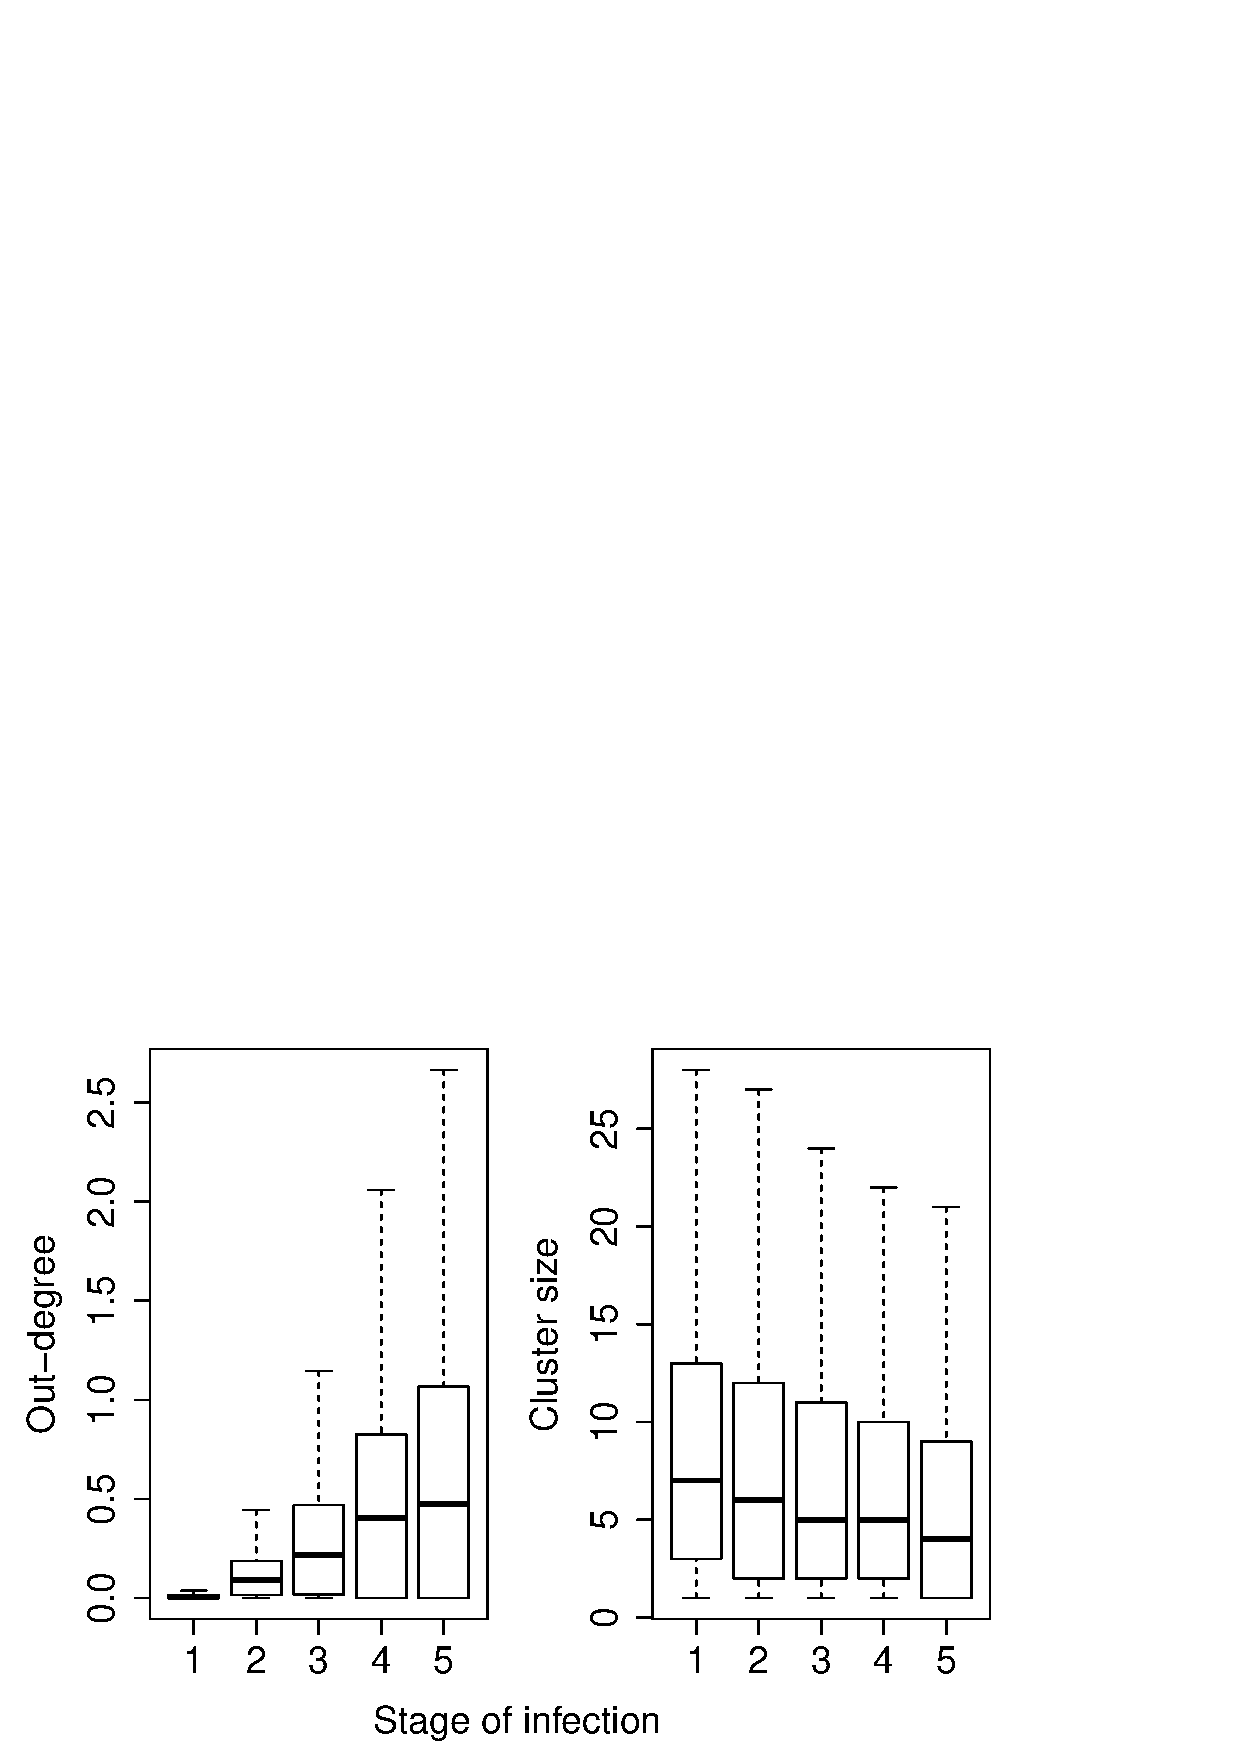
\includegraphics[width=\textwidth]{\figures/bp_base-3.pdf}        
        \label{fig1b}
    \end{subfigure}
    
    \begin{subfigure}[b]{0.45\textwidth}
        \caption{}
        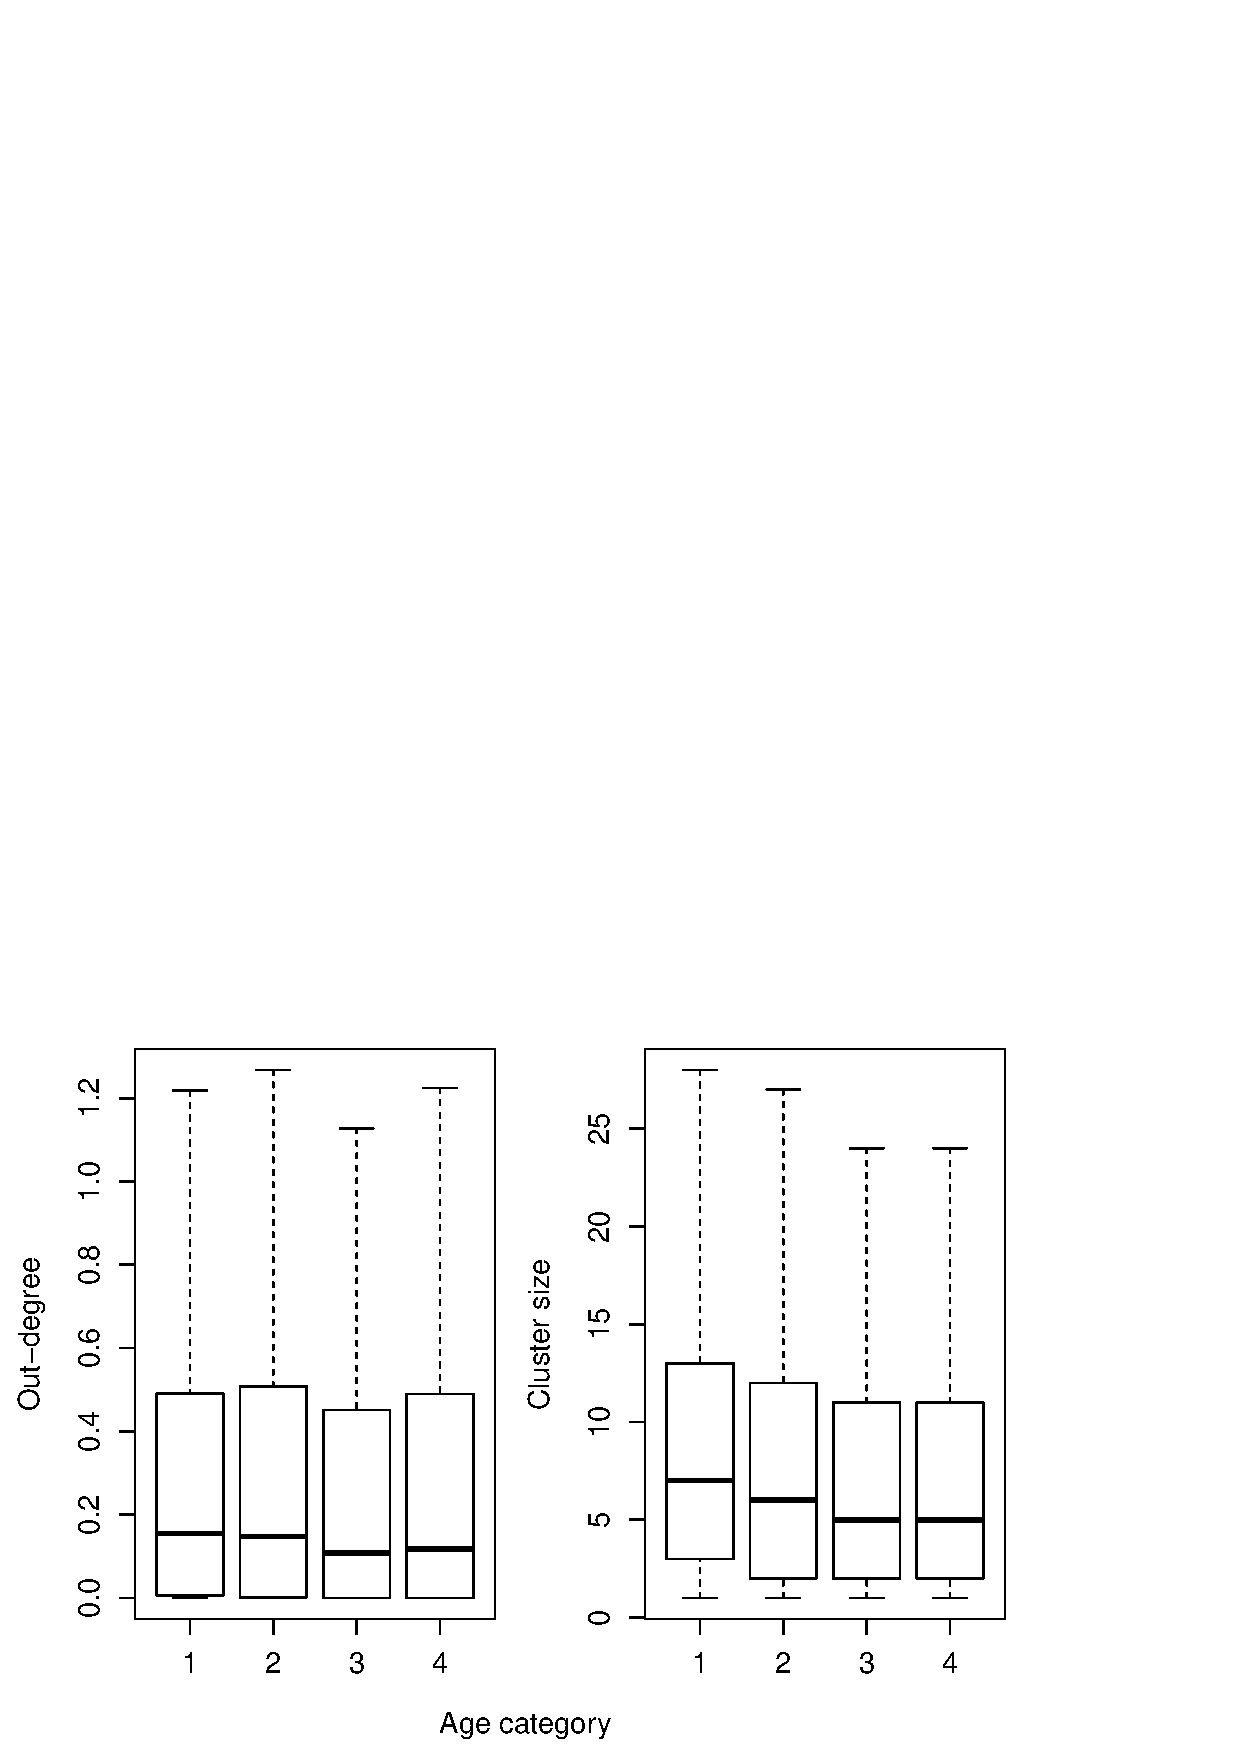
\includegraphics[width=\textwidth]{\figures/bp_base-2.pdf}        
        \label{fig1c}
    \end{subfigure}
   \caption[Distribution of out-degrees and cluster sizes by covariates]{Distribution of out-degrees and cluster sizes by (a) risk level: transmission rate was defined in the model as 10 times higher for risk level 2 relative to risk level 1; (b) stage of infection: relative transmission rates in the model were respectively 10, 1, 1, 1 and 3 for stages 1 to 5 of infection; (c) age category: transmission rates were equal for all 4 age categories in the model. Values are aggregated from 100 simulation replicates. Outliers are not shown. Distance threshold for clustering algorithm is 1.5\%.}
   \label{fig1}
\end{figure}

%-------------


\begin{figure}
    \centering
    \begin{subfigure}[b]{0.45\textwidth}
        \caption{}
        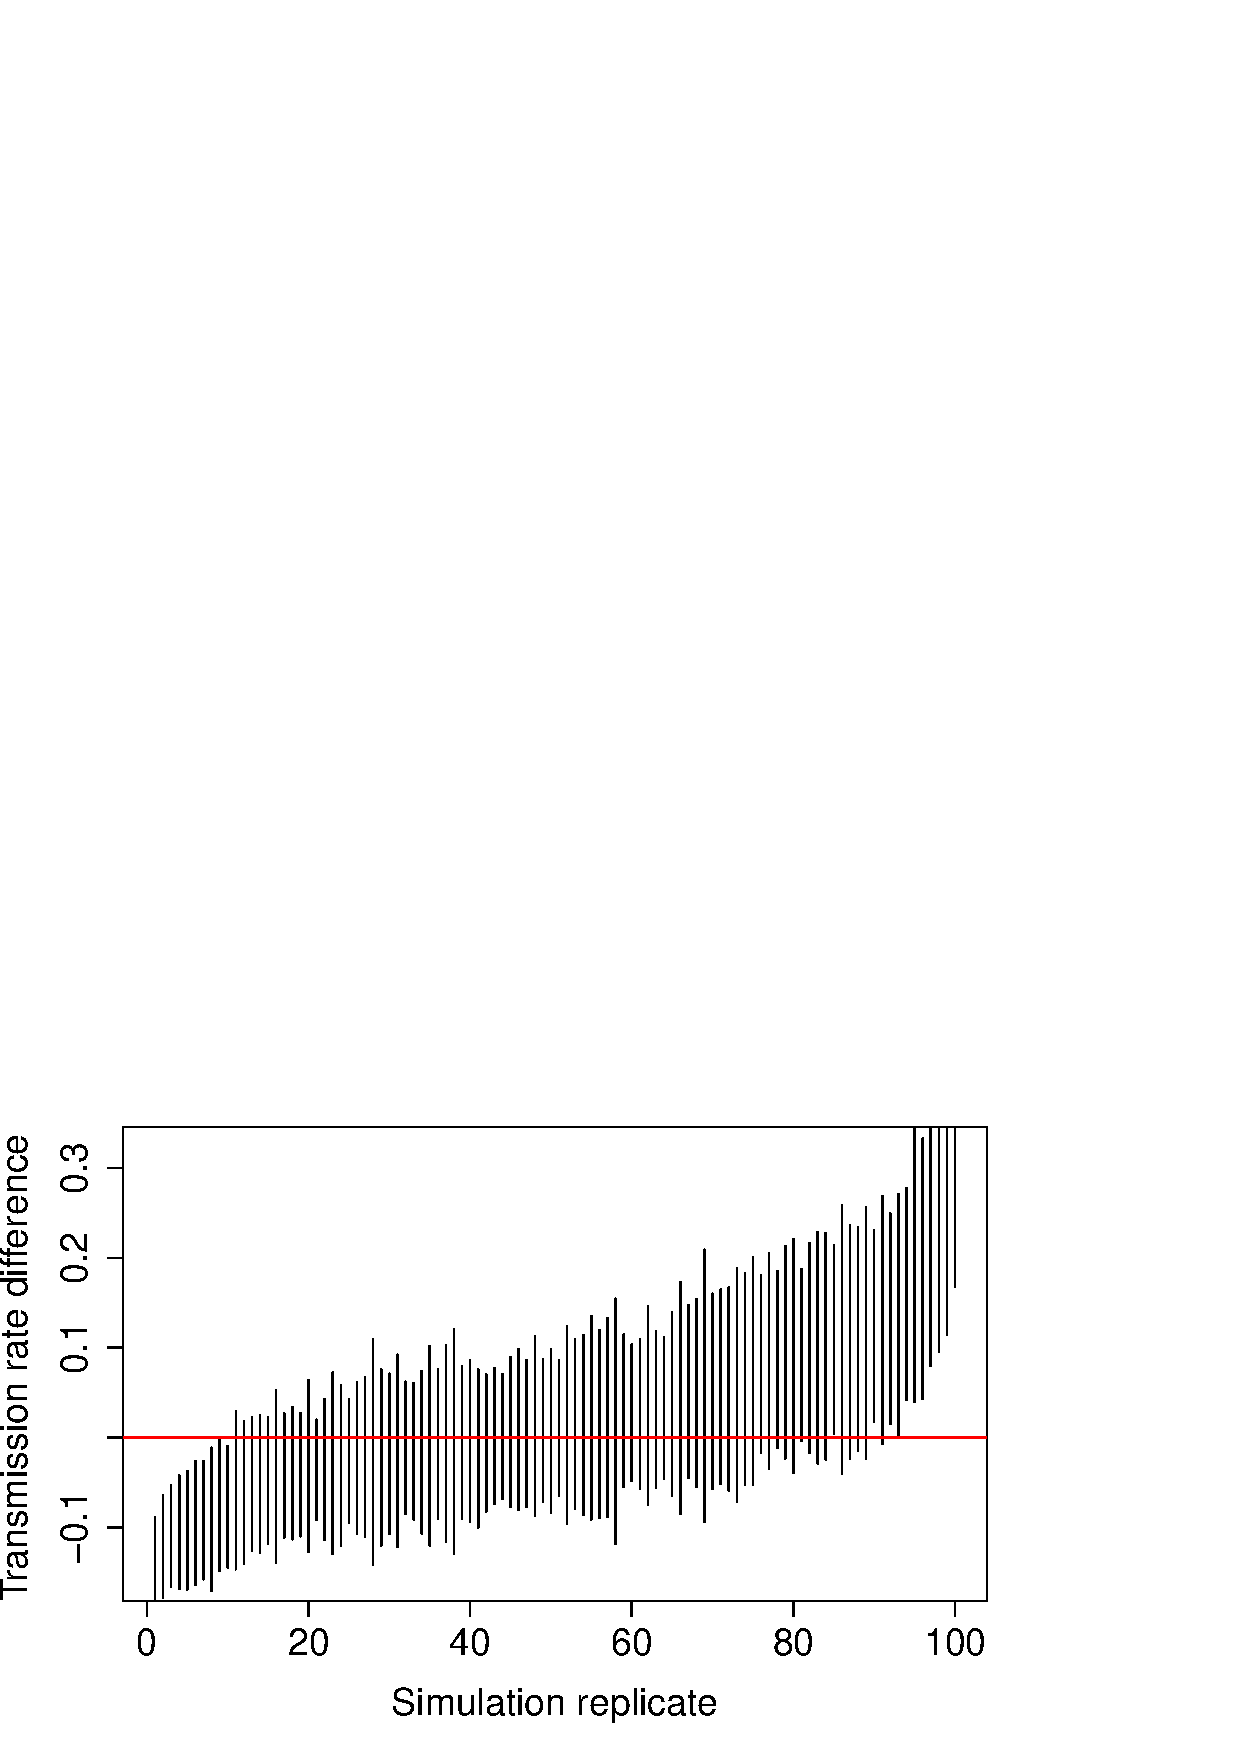
\includegraphics[width=\textwidth]{\figures/plot_rate_diff-1.pdf}
        \label{fig3a}
    \end{subfigure}
    ~ 
    \begin{subfigure}[b]{0.45\textwidth}
        \caption{}
        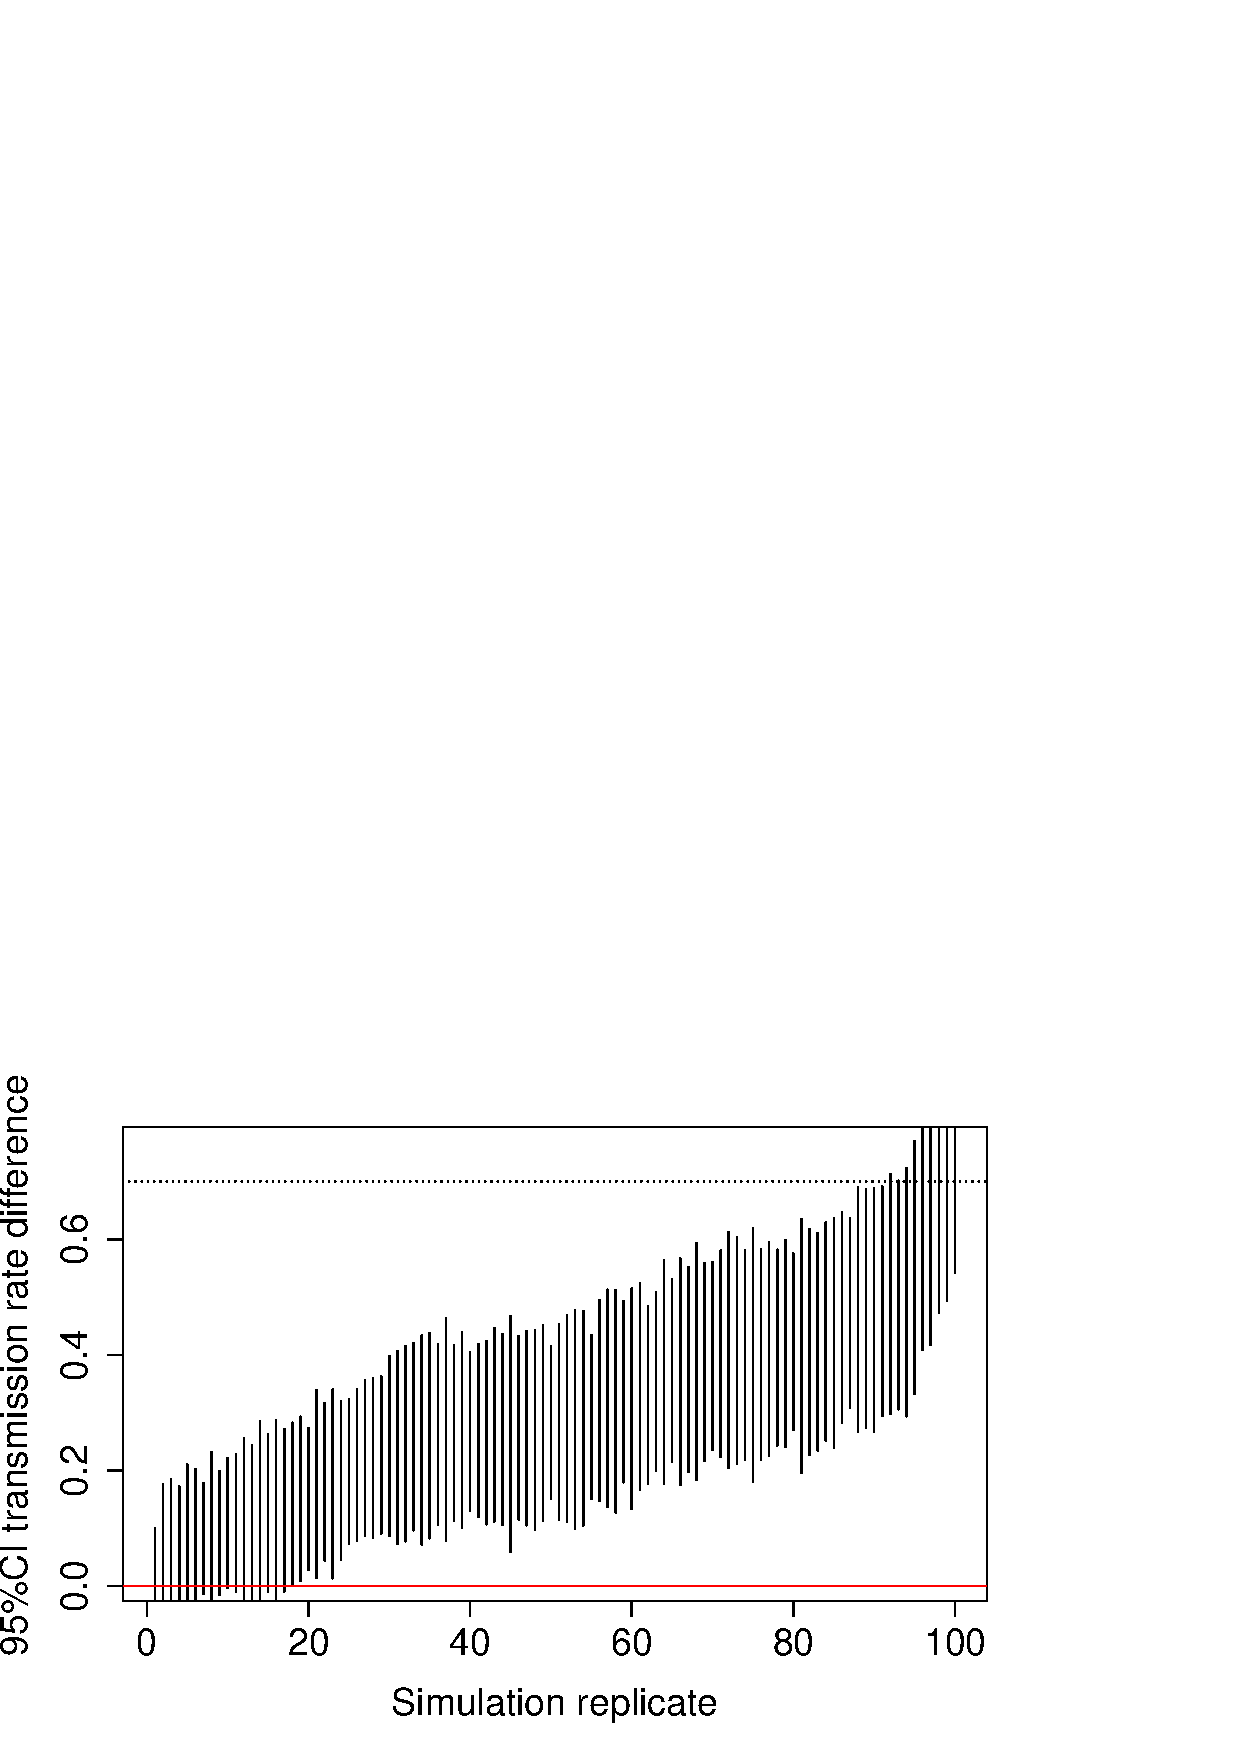
\includegraphics[width=\textwidth]{\figures/plot_rate_diff-2.pdf}        
        \label{fig3b}
    \end{subfigure}
    
    \begin{subfigure}[b]{0.45\textwidth}
        \caption{}
        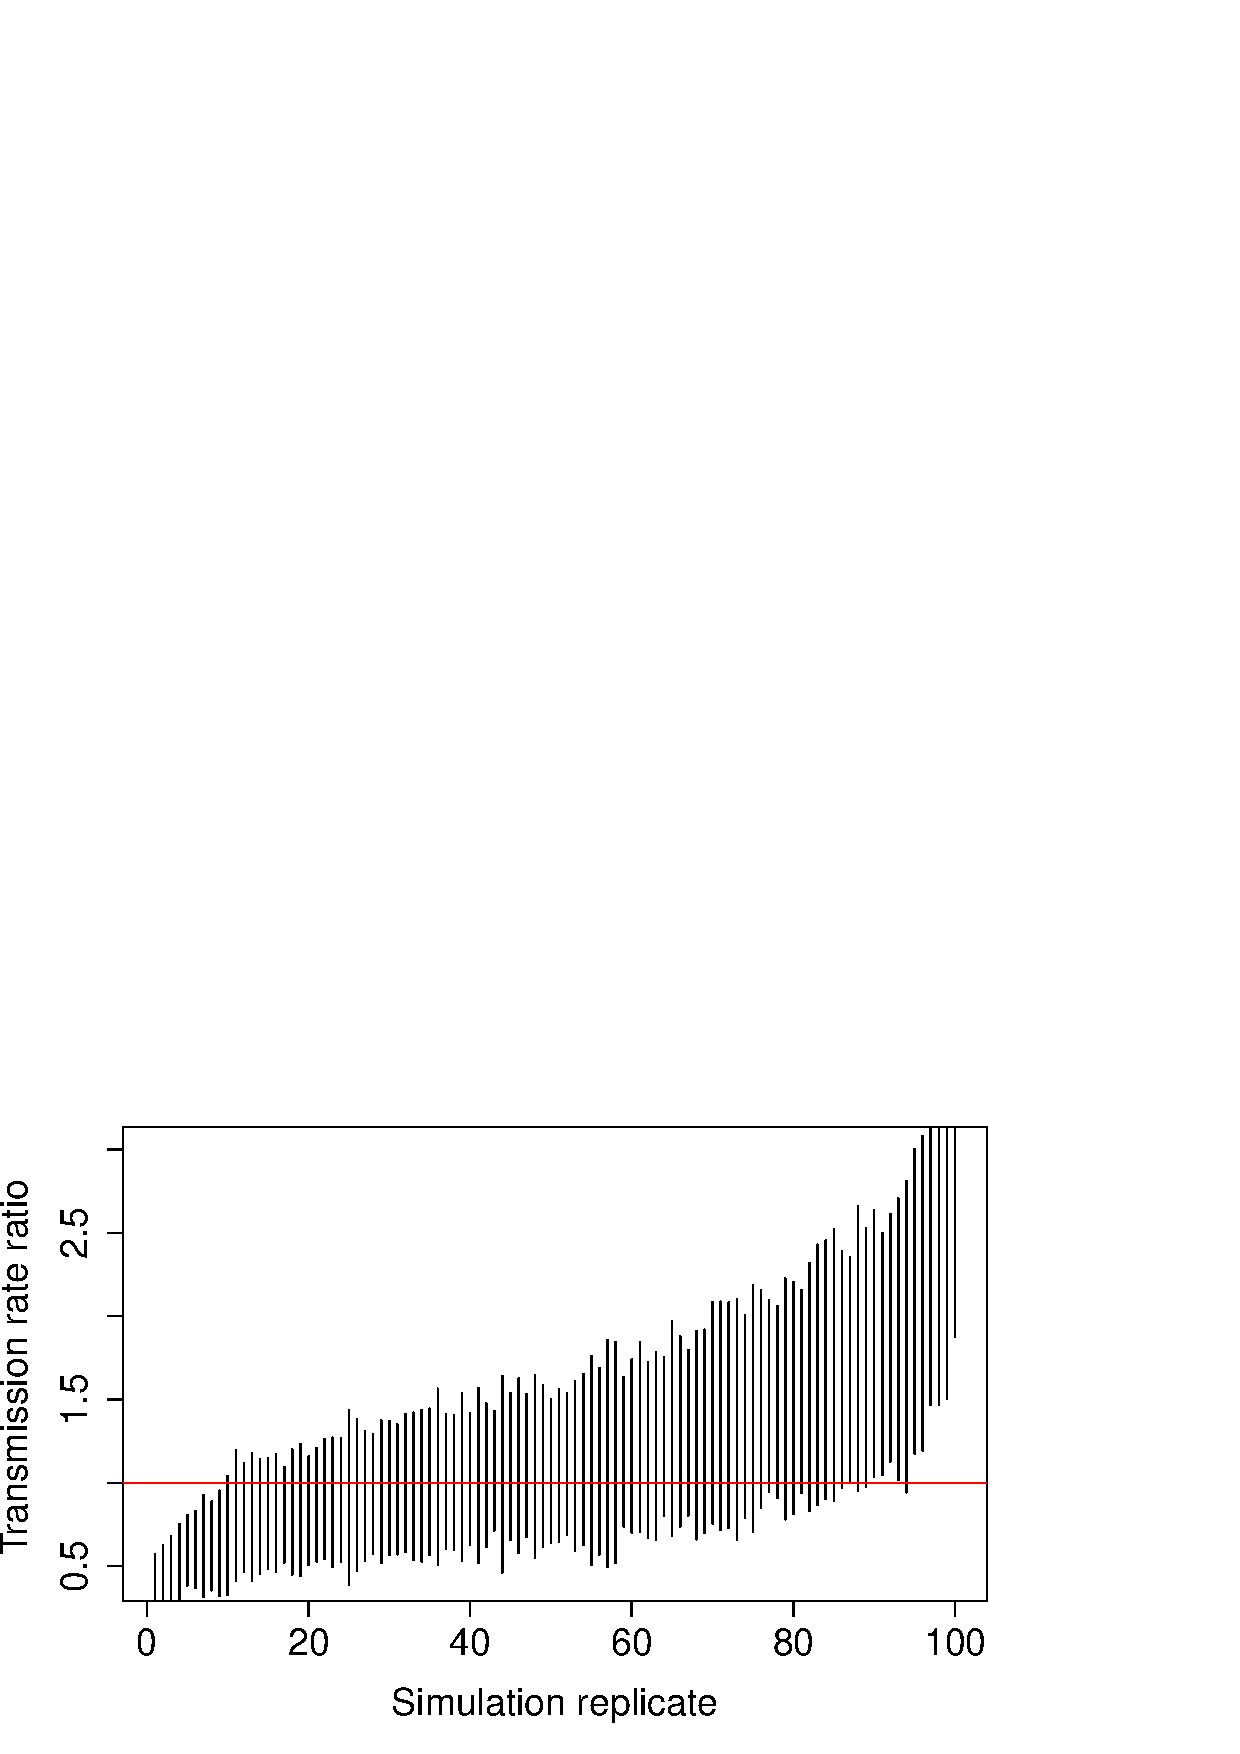
\includegraphics[width=\textwidth]{\figures/plot_rate_ratio-1.pdf}        
        \label{fig3c}
    \end{subfigure}
    ~
     \begin{subfigure}[b]{0.45\textwidth}
        \caption{}
        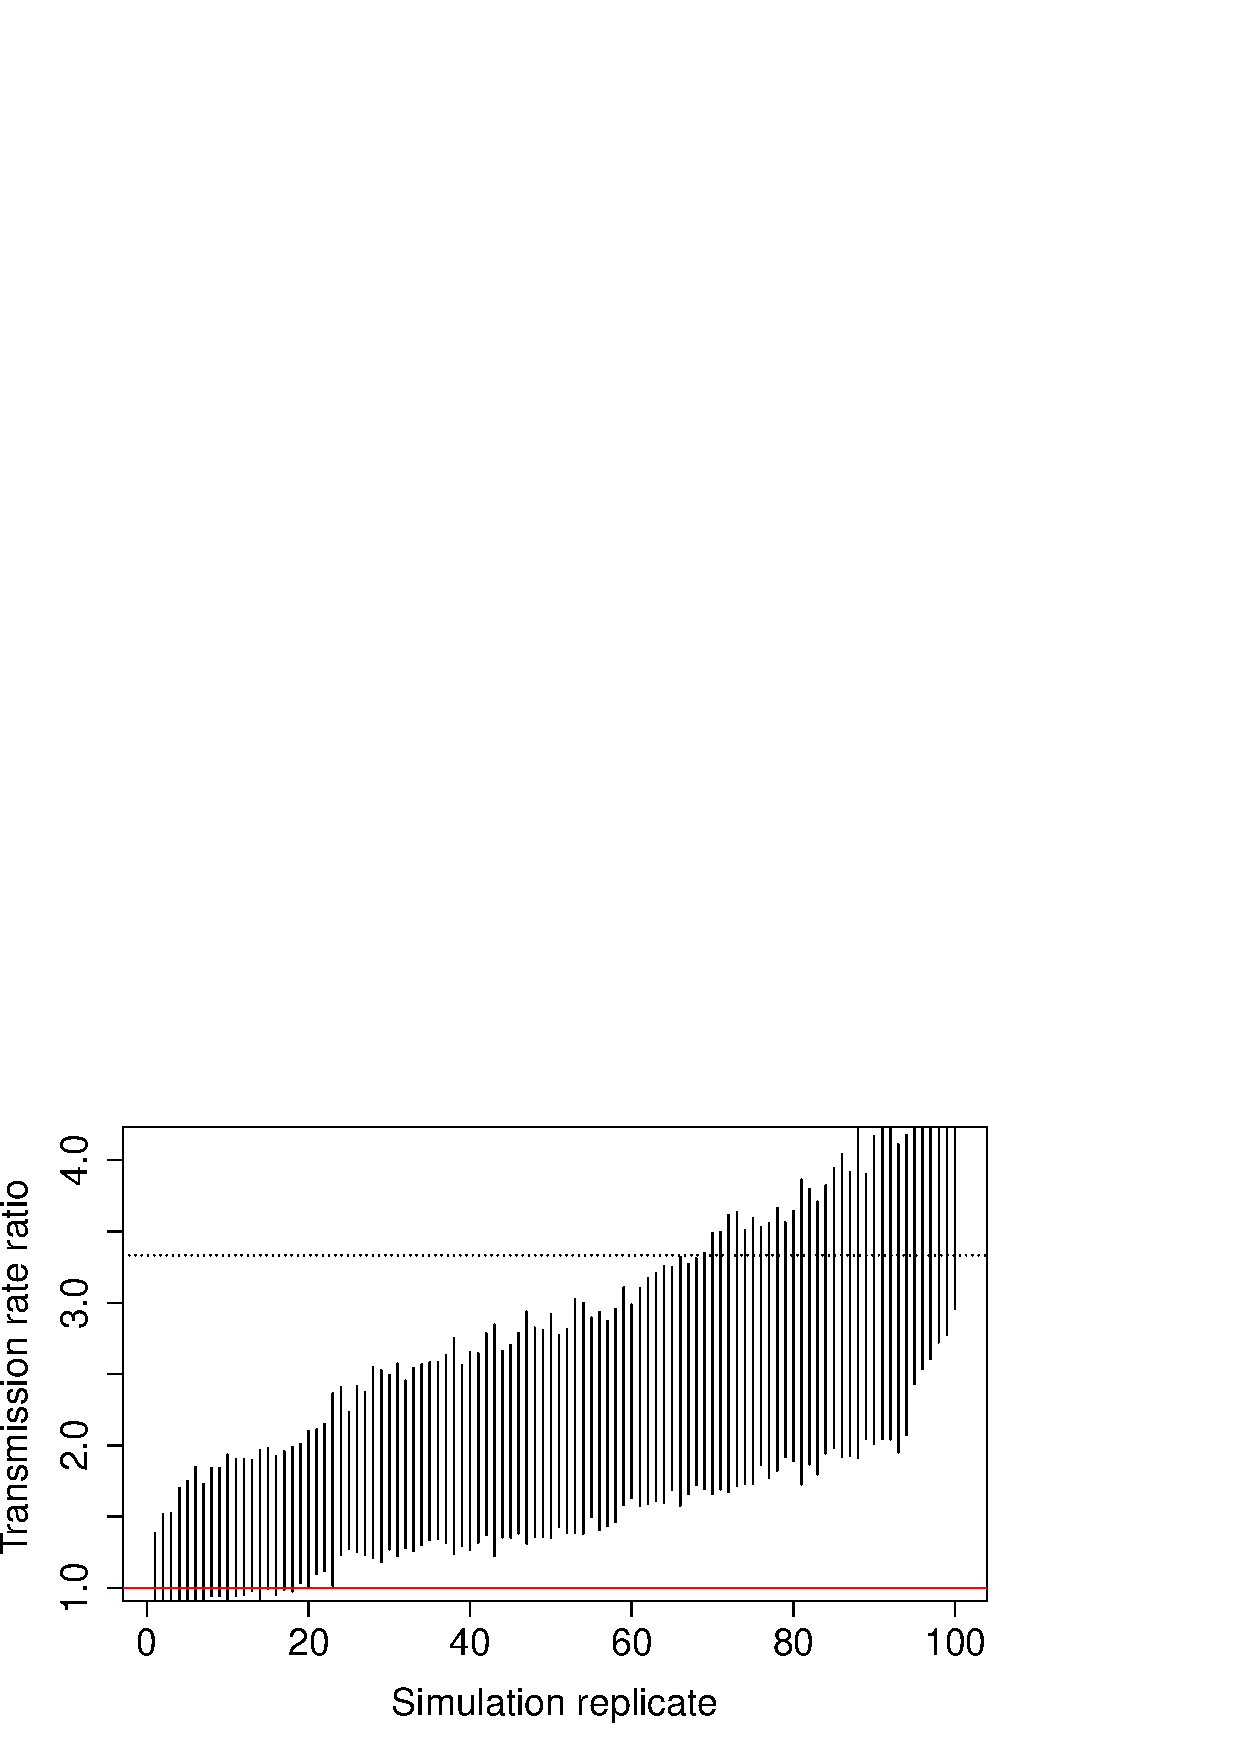
\includegraphics[width=\textwidth]{\figures/plot_rate_ratio-2.pdf}        
        \label{fig3d}
    \end{subfigure}
   \caption[Confidence intervals of difference and ratio of transmission rates between early and late stages of infection estimated by source attribution]{Confidence intervals of difference and ratio of transmission rates between early and late stages of infection estimated by source attribution. First row presents estimates of rate difference and second row rate ratio. Left column shows results for the 'equal-rate' scenario where true value is 0 in (a) and 1 in (c), highlighted in red. Right column shows results for the 'baseline' scenario with true values indicated by dotted line. The results of 100 simulation replicates are sorted in increasing order of the median of rate difference or ratio (x-axis).}
   \label{fig3}
\end{figure}


\end{document}